\subsection{\textit{Low Rank Adaptation} (LoRA)}

Dalam dunia pembelajaran mesin, terutama saat bekerja dengan model berukuran besar, efisiensi parameter menjadi salah satu tantangan utama. LoRA, singkatan dari \textit{Low Rank Adaptation}, muncul sebagai solusi untuk tantangan ini dalam konteks \textit{transfer learning}.

Konsep dasar di balik LoRA adalah ide bahwa adaptasi model untuk tugas baru tidak selalu memerlukan perubahan besar pada seluruh parameter model. Sebaliknya, perubahan kecil pada representasi tertentu dapat menghasilkan peningkatan kinerja yang signifikan. Dengan fokus pada \textit{low rank adaptation}, LoRA mengubah hanya sebagian kecil dari bobot model, sementara sebagian besar bobot lainnya tetap tidak berubah. Ini berarti bahwa hanya "sebagian" dari informasi dalam model yang diperbarui, yang mengarah pada efisiensi komputasi yang meningkat \parencite{lora}.

\begin{figure}[ht]
    \centering
    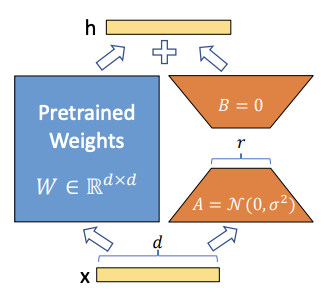
\includegraphics[width=0.8\textwidth]{chapter-2/lora.png}
    \caption{Arsitektur LoRA \parencite{lora}}
    \label{fig:lora}
\end{figure}

Salah satu kelebihan utama dari pendekatan ini adalah kemampuannya untuk mengurangi \textit{overhead} komputasi. Dalam praktiknya, ini berarti bahwa waktu pelatihan dan sumber daya yang diperlukan untuk adaptasi model menjadi jauh lebih sedikit dibandingkan dengan metode lain yang mungkin melibatkan pelatihan ulang model dari awal atau menambahkan sejumlah besar parameter tambahan.

Pendekatan LoRA menjadi sangat relevan dan berharga, terutama saat berhadapan dengan model-model berukuran besar seperti GPT-3. Model-model seperti ini memiliki jumlah parameter yang sangat besar, sehingga pelatihan ulang atau menambahkan parameter tambahan bisa menjadi sangat mahal dari segi komputasi. Dengan LoRA, adaptasi model-model besar menjadi lebih praktis dan dapat dilakukan dengan efisiensi yang jauh lebih tinggi, tanpa mengorbankan kinerja.

Dengan demikian, LoRA menawarkan pendekatan yang menjanjikan untuk mengadaptasi \textit{pre-trained model} dengan cara yang lebih efisien, memungkinkan peneliti dan praktisi untuk memanfaatkan kekuatan model berukuran besar tanpa harus berurusan dengan beban komputasi yang berat.